\documentclass[english]{article}
\usepackage[T1]{fontenc}
\usepackage{babel}
\usepackage{graphicx}
\usepackage{physics-patch}
\usepackage[version=4]{mhchem}

\graphicspath{ {./Images/} }

\begin{document}

\section*{Jacobi Coordinates for \ce{Ar-HF}}

\ce{Ar-HF}: we need $3 N - 6 = 3 \cdot 3 - 6 = 3$ coordinates to describe its geometry.

\begin{figure}[h]
	\centering
	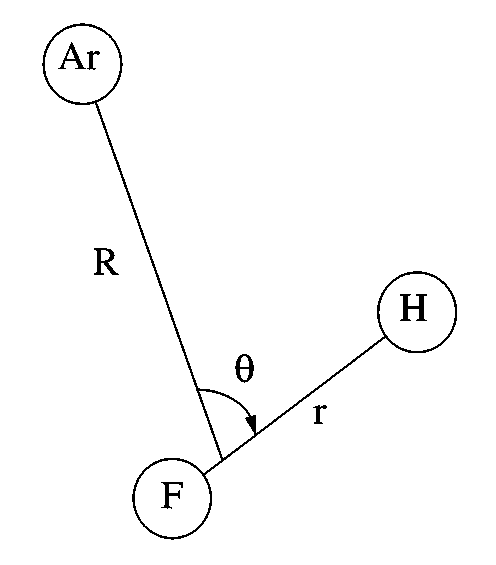
\includegraphics[width=.5\textwidth]{Ar-HF_Jacobi_Coordinates}
\end{figure}

\begin{align}
	\vb{r} & = \vb{r}_{\ce{F}} - \vb{r}_{\ce{H}} \\
	\vb{r}_\mathrm{CM}^{\ce{HF}} & = \frac{m_{\ce{H}} \vb{r}_{\ce{H}} + m_{\ce{F}} \vb{r}_{\ce{F}}}{m_{\ce{H}} + m_{\ce{F}}} \\
	\vb{R} & = \vb{r}_{\ce{Ar}} - \vb{r}_\mathrm{CM}^{\ce{HF}} \\
	\theta & = \arccos{\frac{\vb{r} \vdot \vb{R}}{r R}}
\end{align}

If we fix~$r$, we are left with just two coordinates, $(R, \theta)$.

\end{document}
